\section{Teil 1: Bohr'sches Magneton}
  \subsection{Hysterese-Effekt}
    Mit dem Teslameter wird die Stärke des Magnetfeldes zwichen den Spulen bei 6 Stromstärken, von \SI{8}{\ampere} bis \SI{13}{\ampere}, gemessen. Für den Fehler nehmen wir \SI{0.1}{\ampere} an. Der Hysterese-Effekt wird nun eingeschätzt, indem wir den zusammenhang zwischen Stromstärke und Magnetfeld ermitteln. Und wir führen diese Messung bei fallender und steigender Stronstärke durch. Für alle Messpunkte gilt: wir nutzen drei Messwerte und bilden daraus ein Mittel. In \hyperref[plot::1]{Abb. \ref*{plot::1}}\\\\
    Die aus den Werten ermittelten linearen Fits ergaben folgende Steigungen:\\\\
    \textbf{bei aufsteigender Stromstärke:}
      \begin{align}
        m_u = \SI{39.461+-2.198}{\milli\tesla\per\ampere}
      \end{align}
    \textbf{bei absteigender Stromstärke:}
      \begin{align}
        m_d = \SI{38.874+-2.192}{\milli\tesla\per\ampere}
      \end{align}\\
    Die beiden Geraden stimmen dabei mit weniger als \SI{1}{\sigma} überein, und in unserem Fall kann der Hsyterese-Effekt vernachlässigt werden. Für die folgenden Berechnungen wird ein Mittel gebildet, es ergibt sich:
    \begin{align}
      B(I) = \SI{39.168+-1.552}{\milli\tesla\per\ampere} \cdot I + \SI{130.765+-15.849}{\milli\tesla}
    \end{align}
    (Die Fehler erhält man mittels Fehlerfortpflanzung)

    \begin{figure}[H]
      \centering
      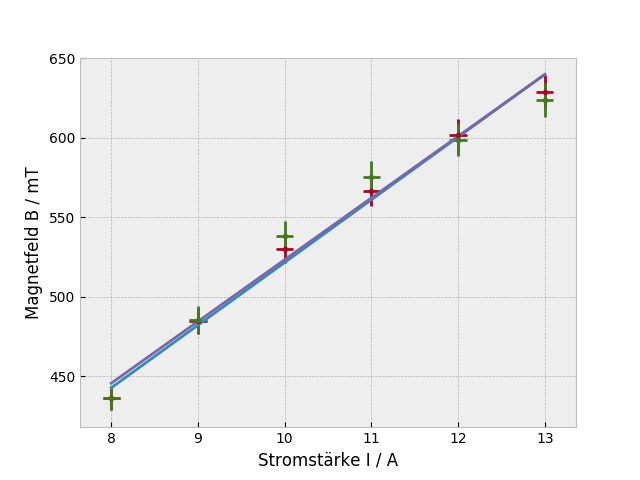
\includegraphics[width=.6\paperwidth]{Auswertung/hysteresis}
      \caption{Hysterese}
      \label{plot::1}
    \end{figure}

  \subsection{Polarisation}
    Das Licht der Cadmium Lampe wird in longitudinaler und transversalter Richtung zum Magnetfeld beobachtet. Durch Verwendung eines linearen Polarisationsfilters und eins $\lambda$/4-Plättchens kann de Polarisation analysiert werden.

    \subsubsection{Beobachtung in longitudinaler Richtung}
      Bei dieser Beobachtungsrichtung sind sowohl mit als auch ohne linearen Polarisationsfilter 2 Linien pro Beugungsordnung zu sehen. Daraus ist zu schließen, dass es sich bei dem Licht um zirkular polarisiertes Licht handelt. (s. \hyperref[pic::1]{Abb. \ref*{pic::1}})

      \begin{figure}[H]
        \centering
        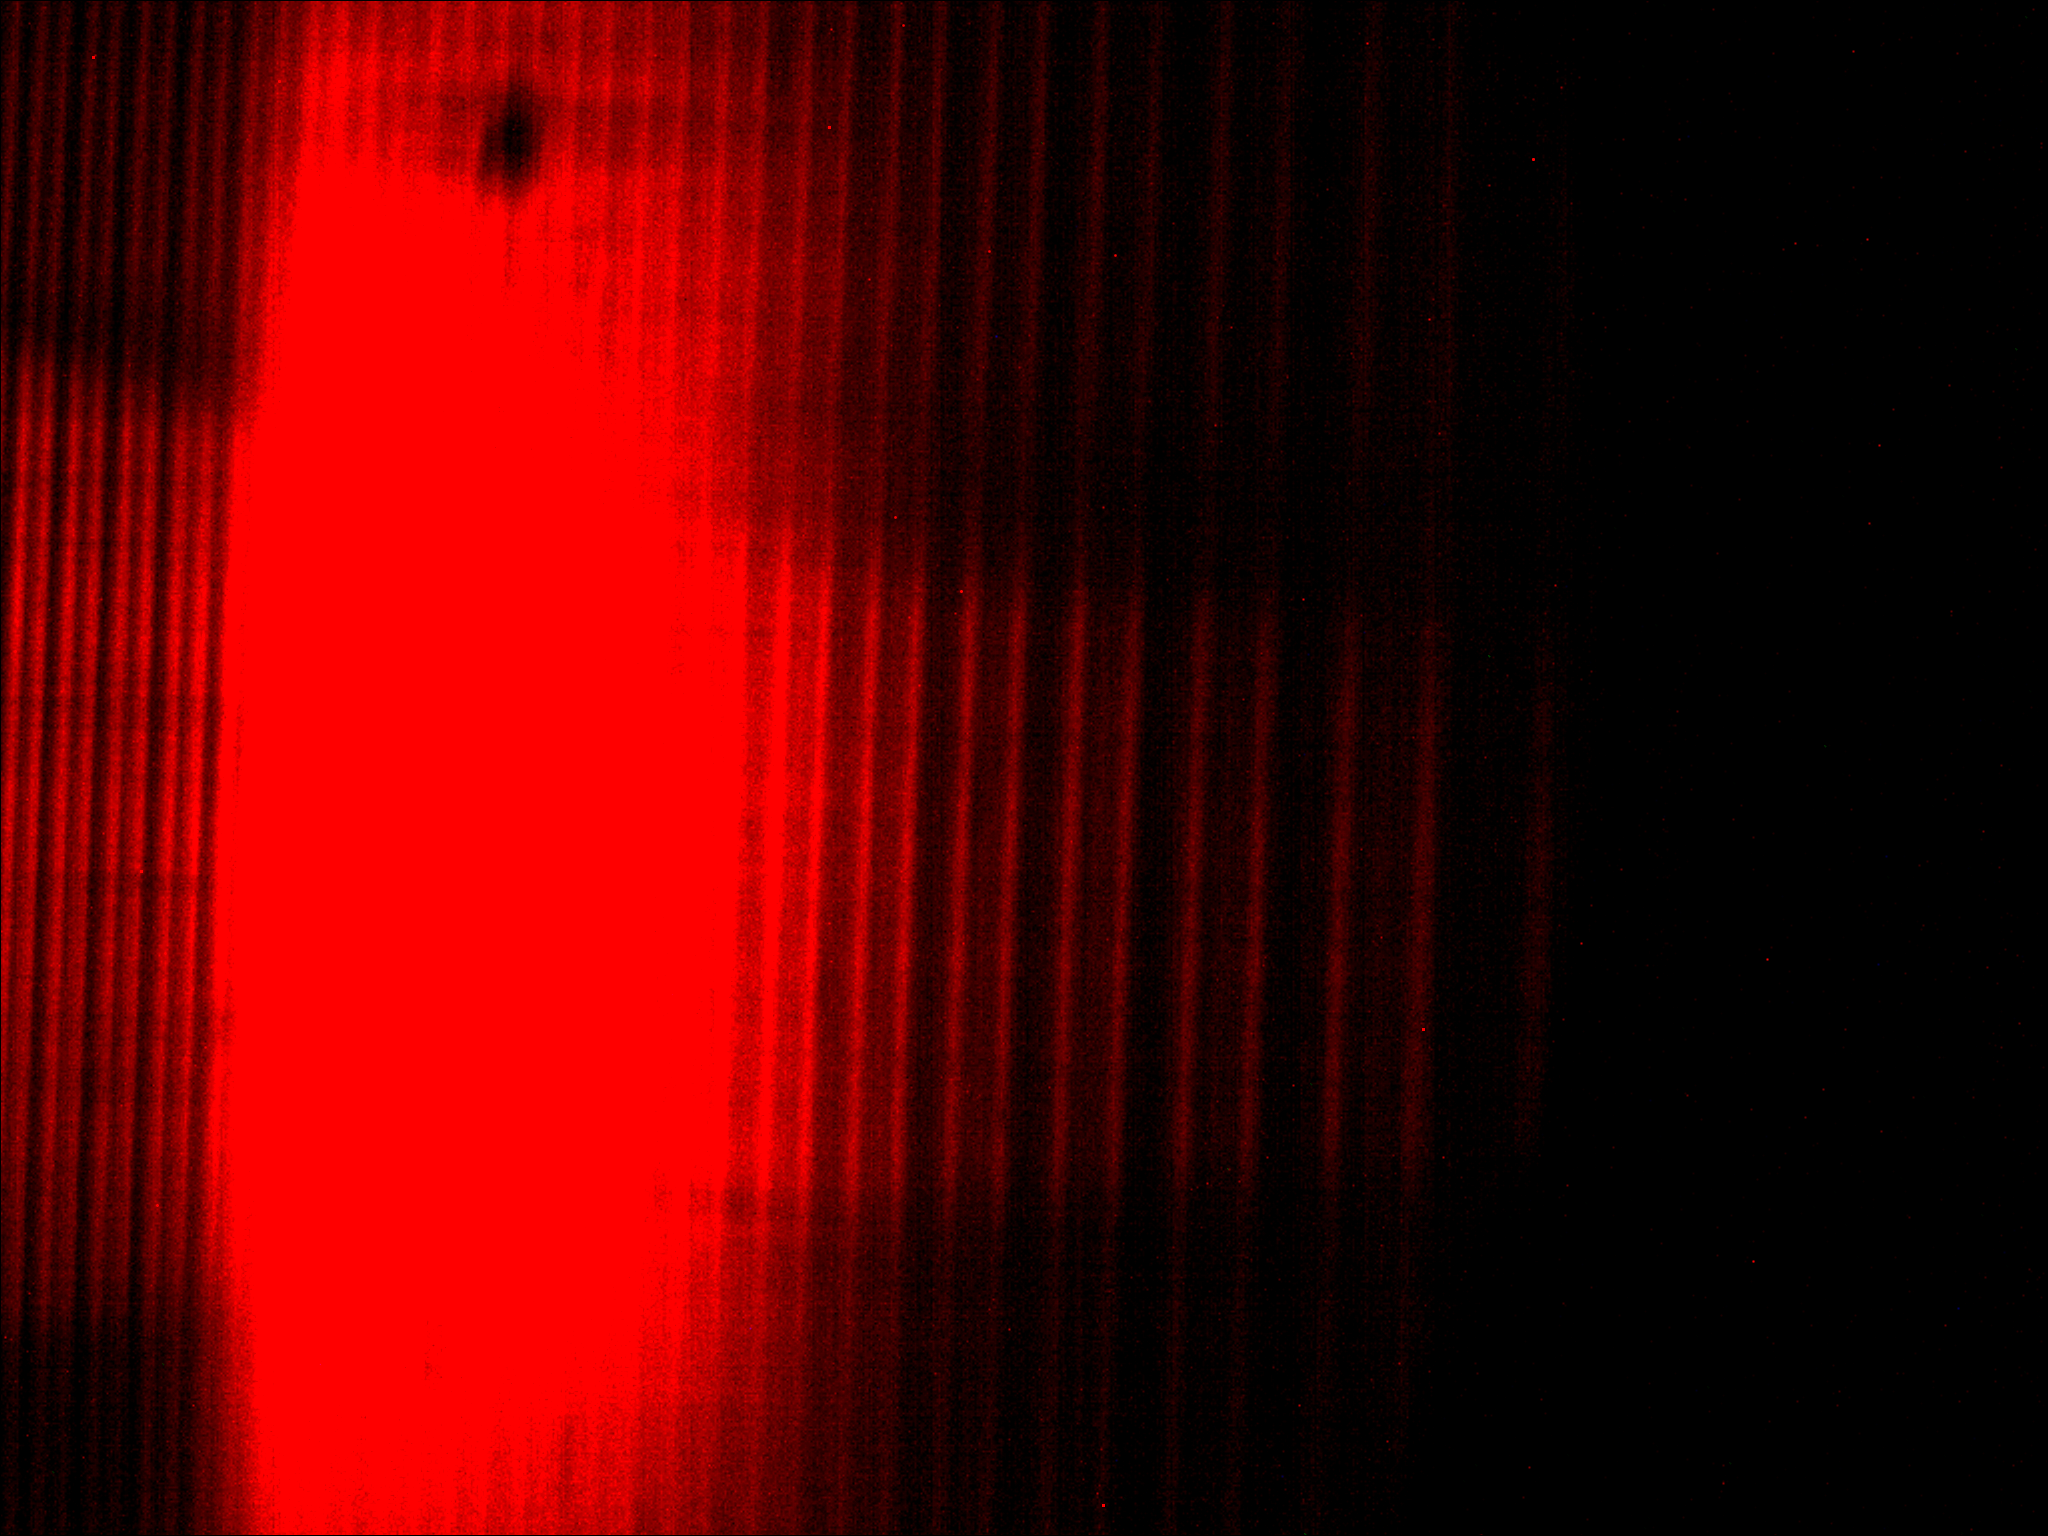
\includegraphics[width=.6\paperwidth, trim={0 200pt 0 400pt}, clip]{Auswertung/data/long/10A_0}
        \caption{Beobachtete Linien in longitudinaler Ausrichtung, ohne Filter}
        \label{pic::1}
      \end{figure}

      Wandelt man nun das Licht mitlilfe des $\lambda$/4-Filters das Licht in linear Polarisiertes um, so kann man mit dem Polarisationsfilter eine der beiden Linien herausfiltern und bei Rotation um \SI{90}{\deg} des $\lambda$/4-Filters die jeweils andere. (s. \hyperref[pic::2]{Abb. \ref*{pic::2}})

      \begin{figure}[H]
        \centering
        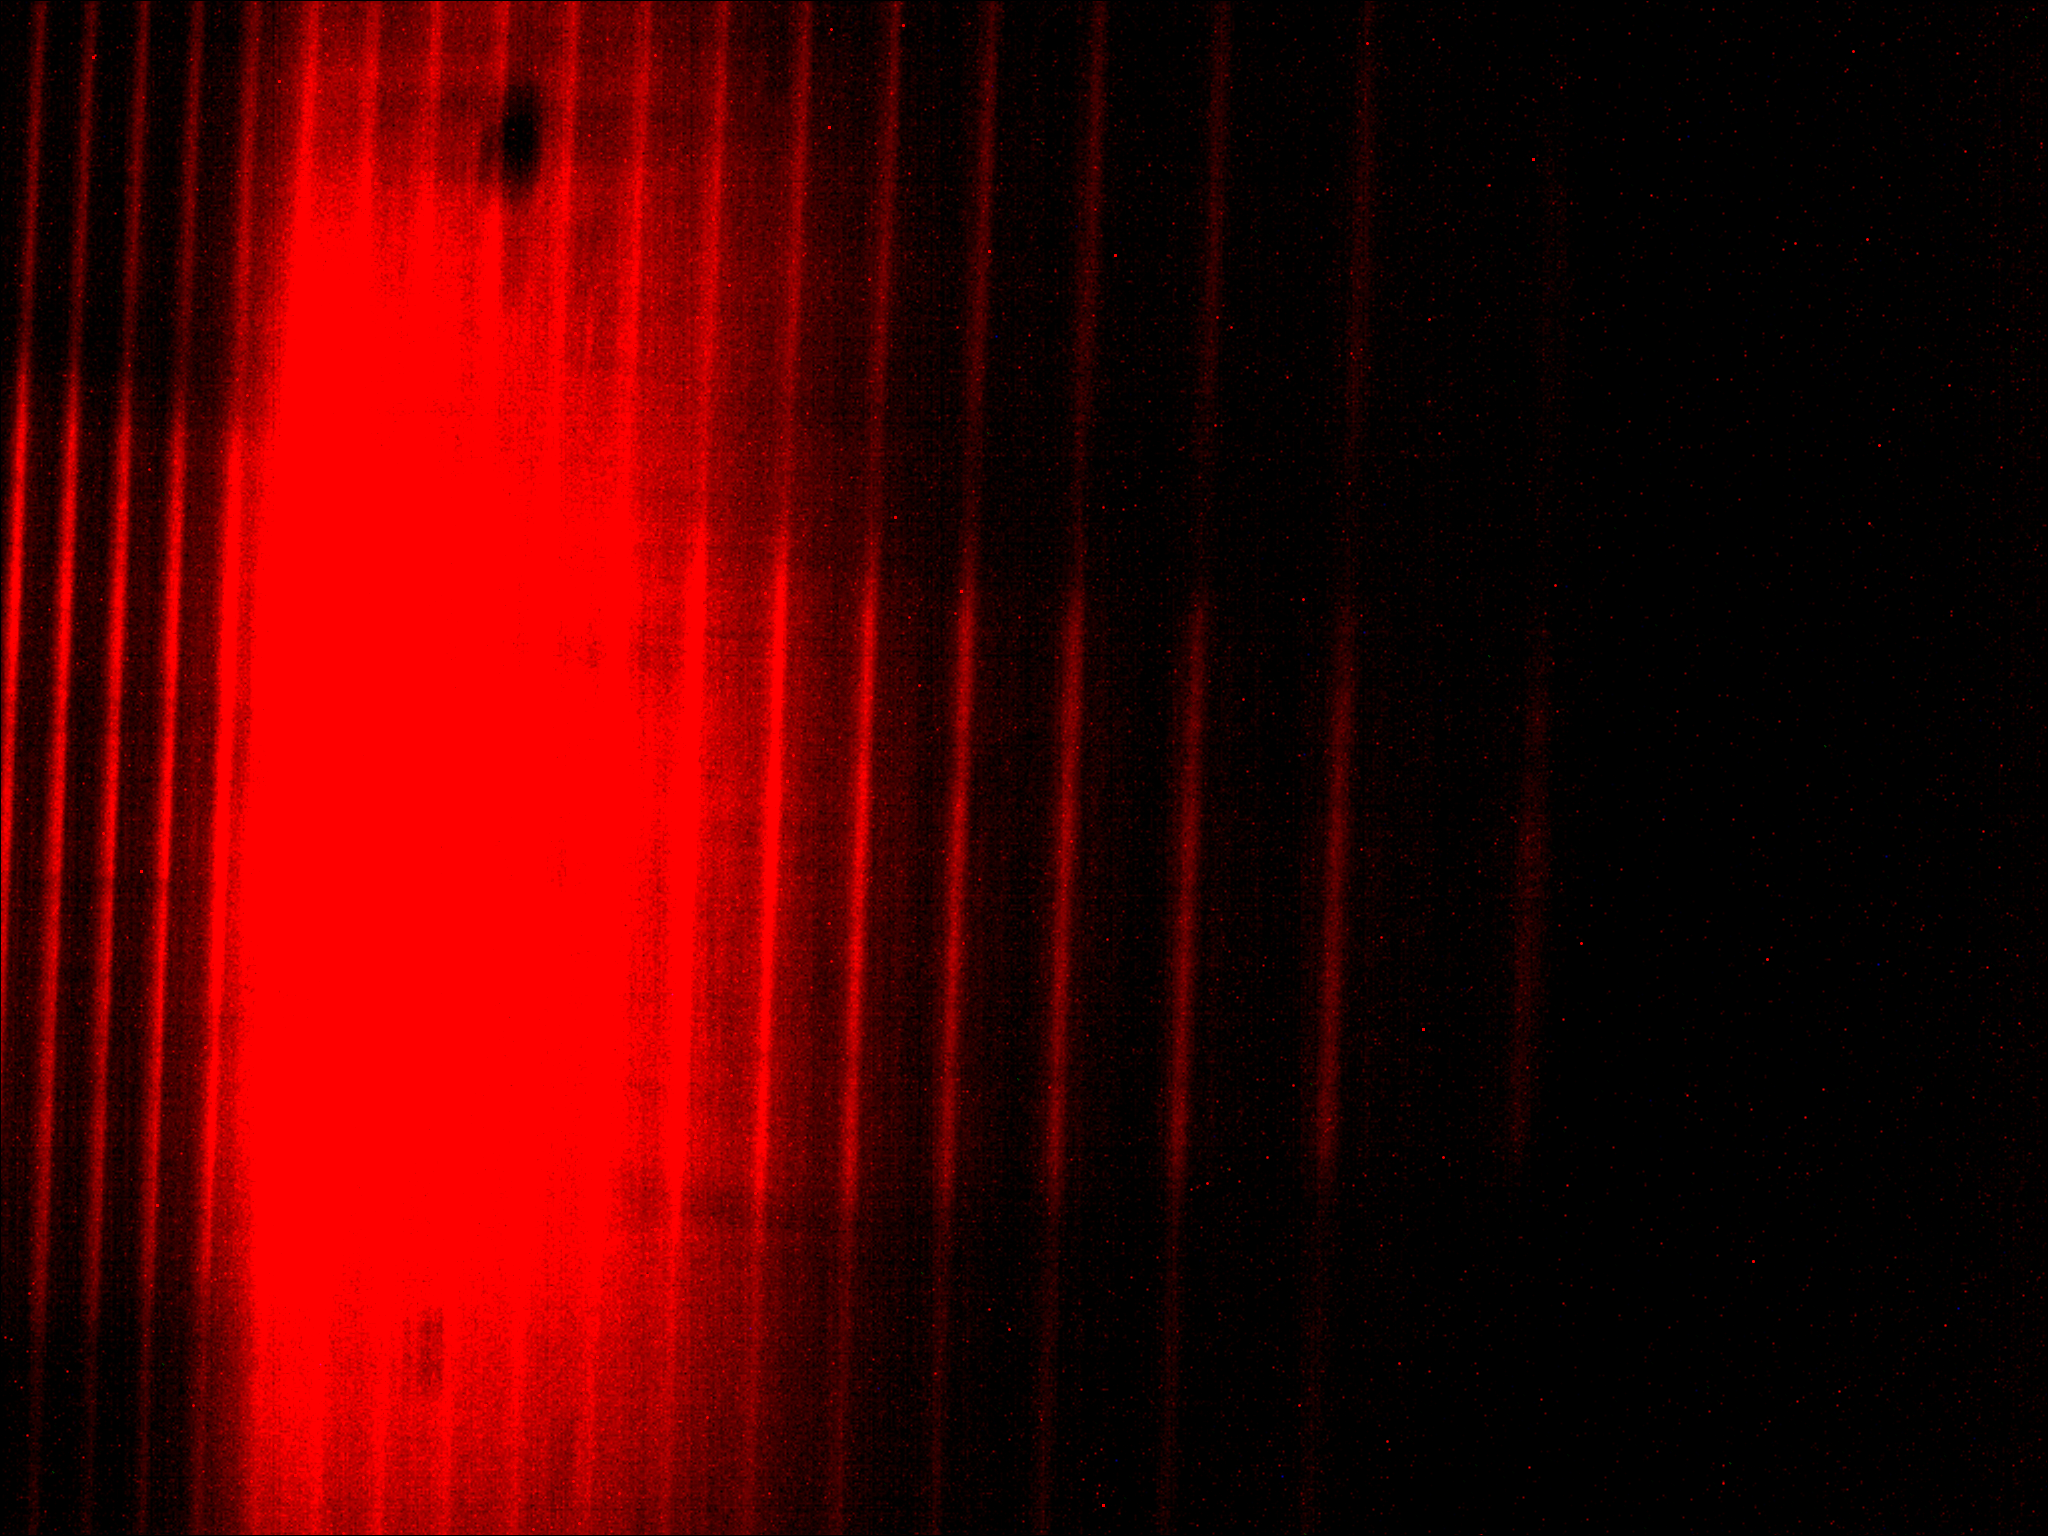
\includegraphics[width=.6\paperwidth, trim={0 650pt 0 200pt}, clip]{Auswertung/data/long/10A_2}
        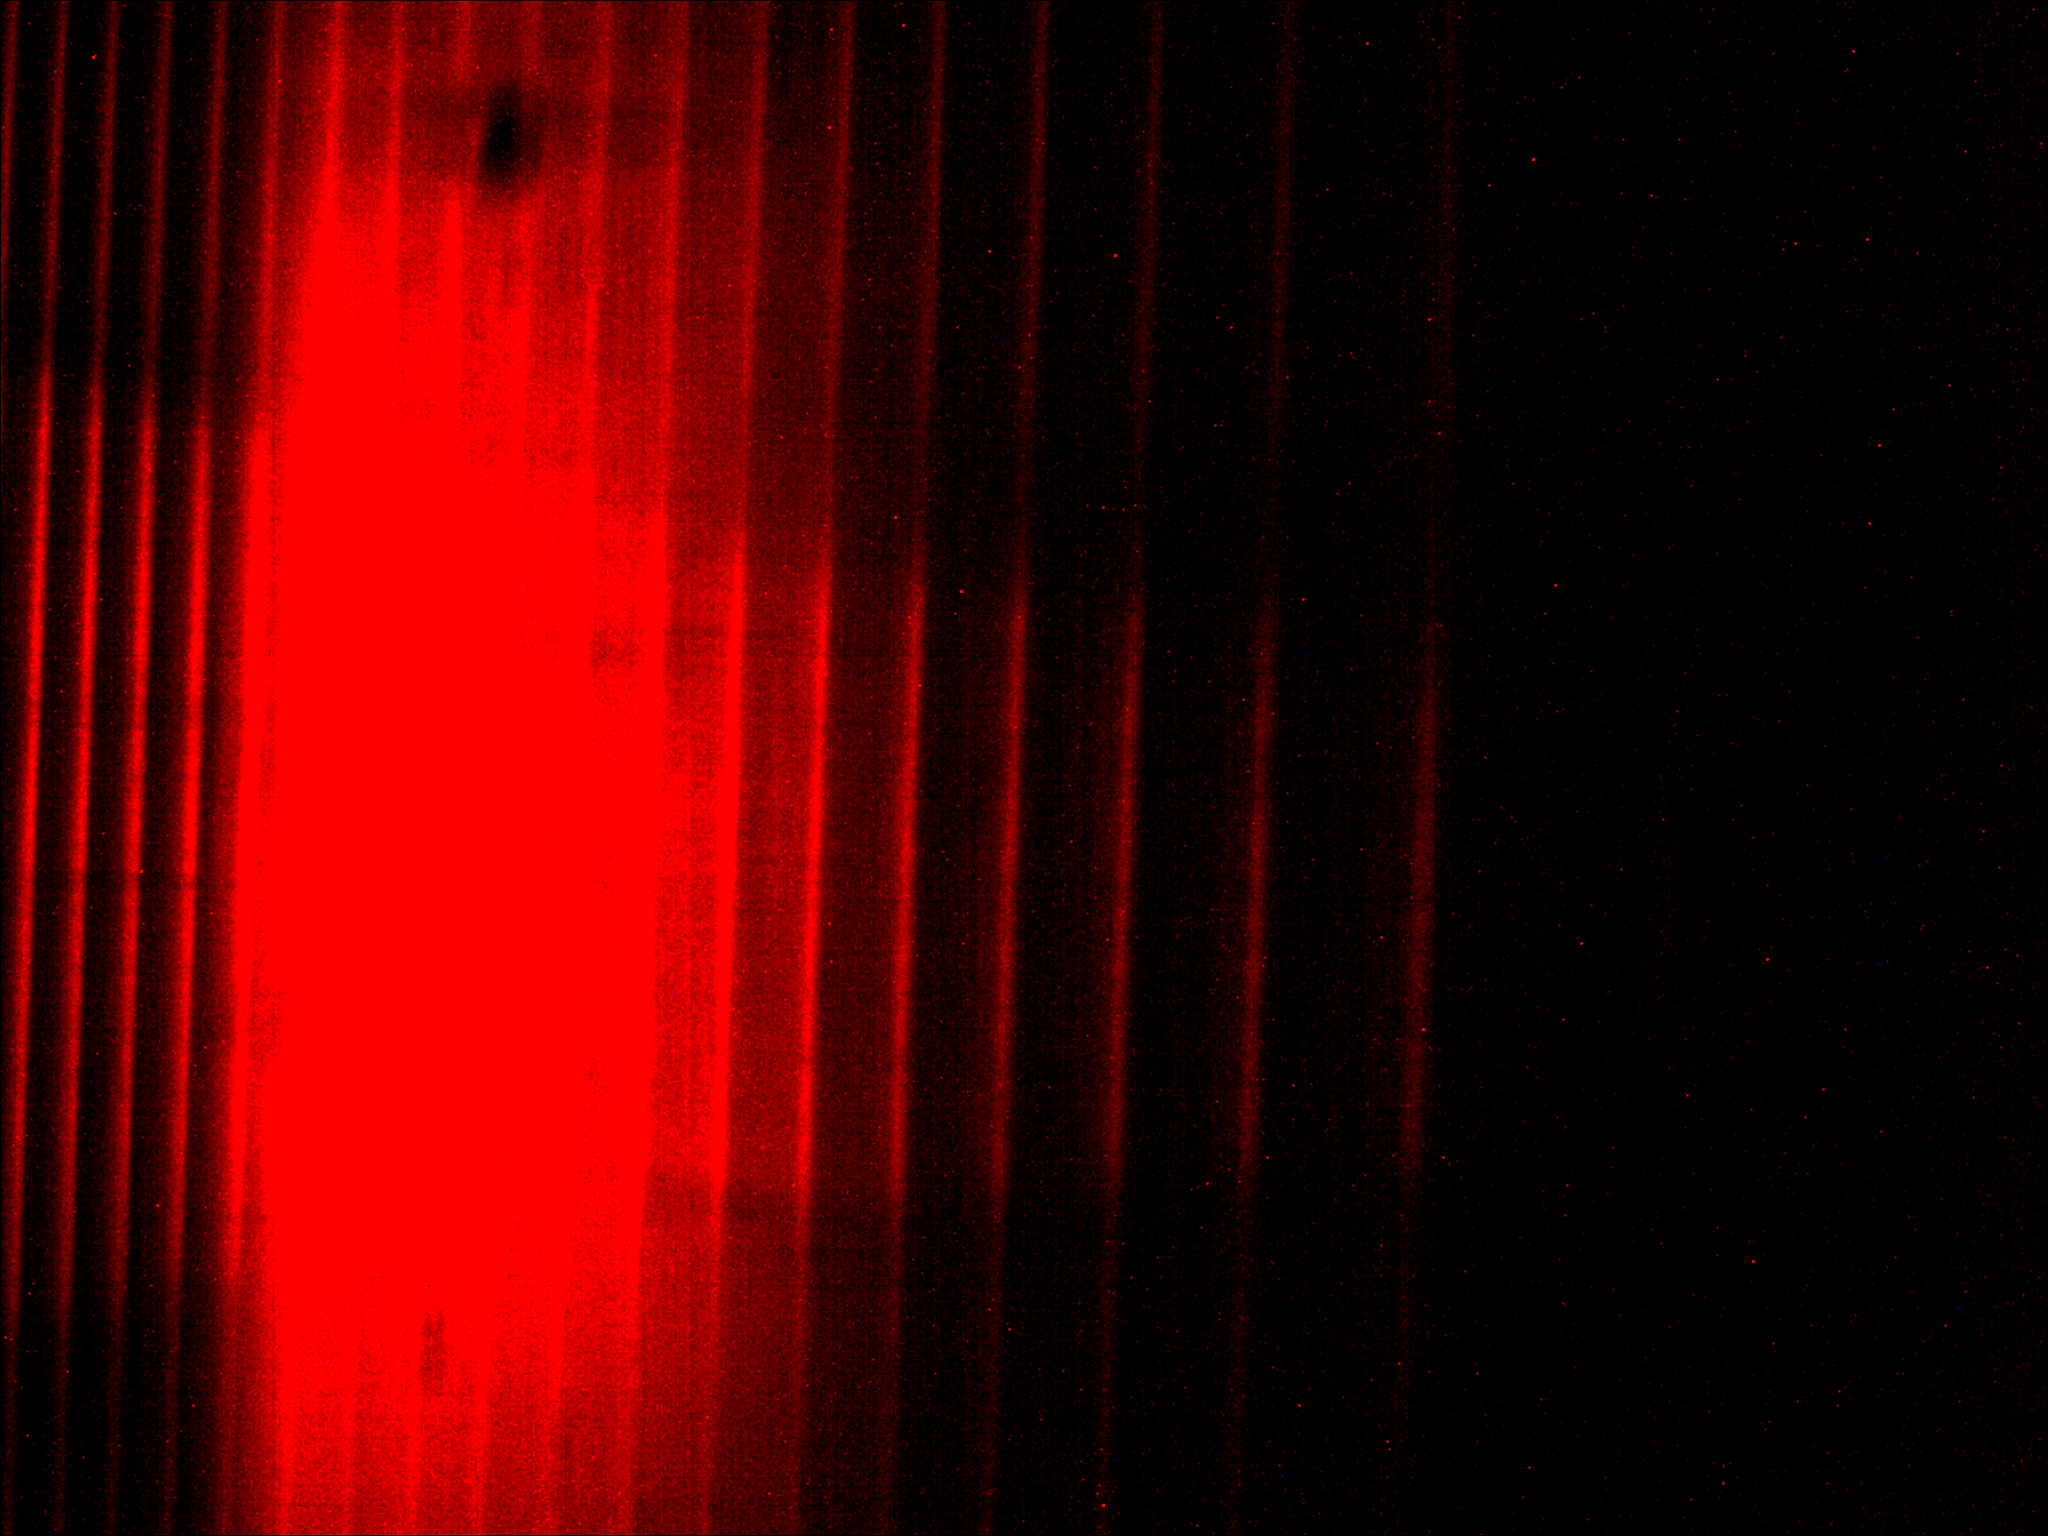
\includegraphics[width=.6\paperwidth, trim={0 0 0 886pt}, clip]{Auswertung/data/long/10A_1}
        \caption{Beobachtete Linien in longitudinaler Richtung, mit $\lambda$/4-Filter und linearem Polarisationsfilter}
        \label{pic::2}
      \end{figure}

    \subsubsection{Beobachtung in transversaler Richtung}
      Hier können wir eine Aufspaltung in drei Linien beobachten. Der Polarisationsfilter lässt entweder die beiden äusseren Linen ($\sigma$-Linien) verschwinden, oder nach einer \SI{90}{\deg} Drehung die mittlere Linie ($\pi$-Linie) (s. \hyperref[pic::3]{Abb. \ref*{pic::3}}). Das Licht ist also linear polarisiert, mit senkrechter Polarisationsrichtung zwichen $\sigma$- und $\pi$-Linien

      \begin{figure}[H]
        \centering
        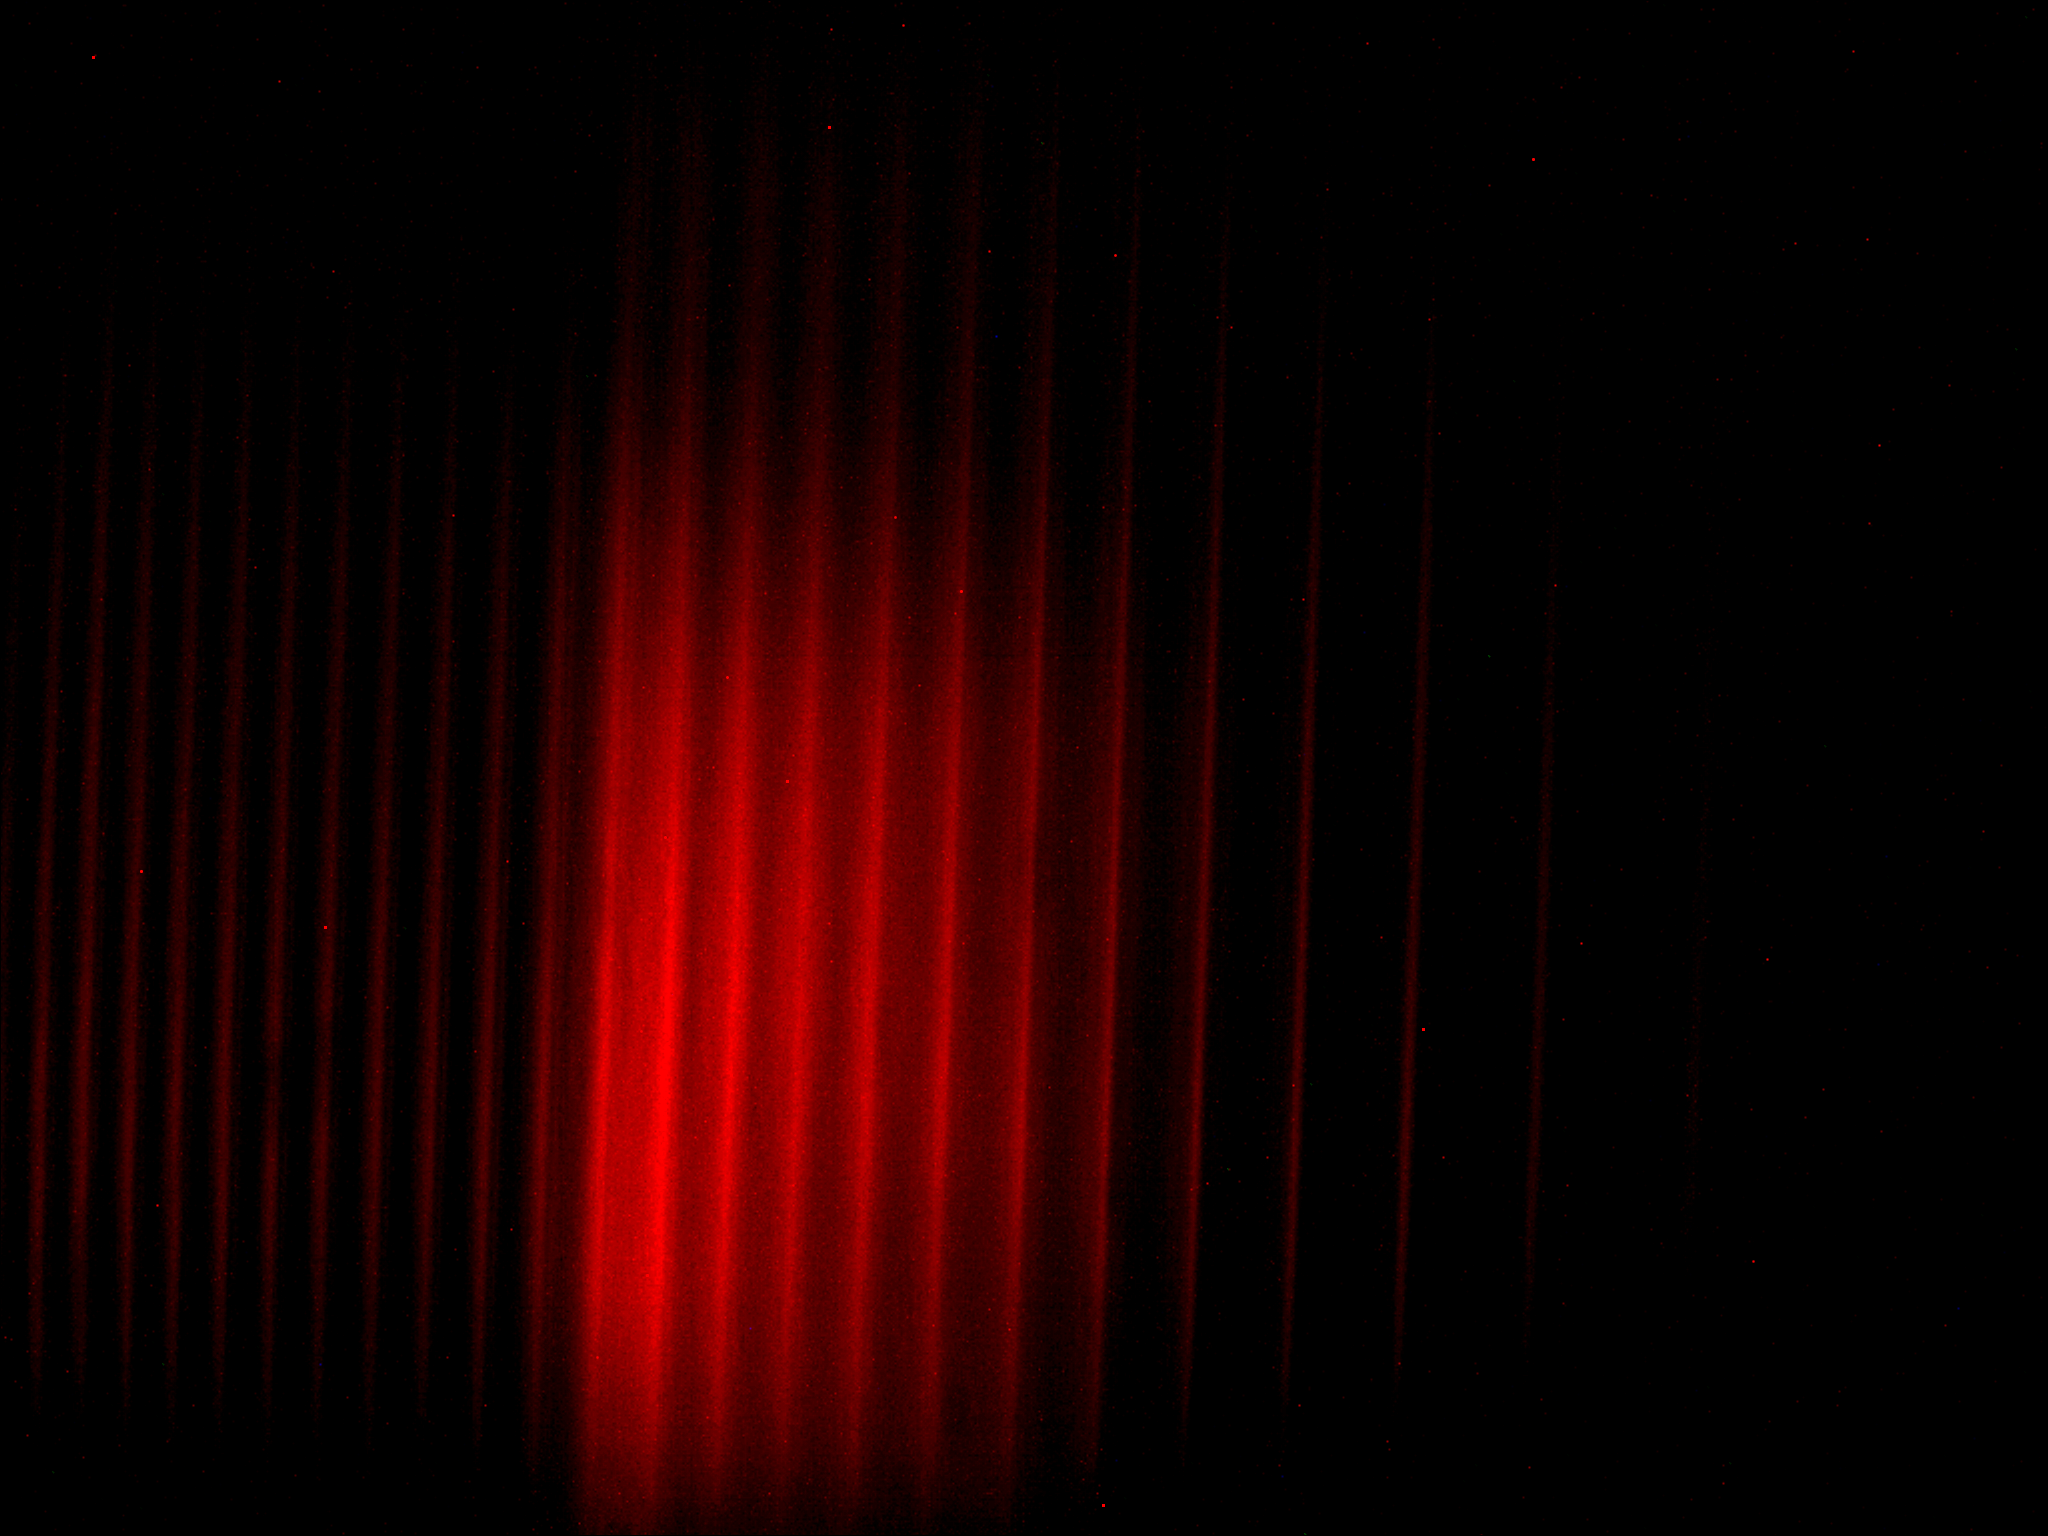
\includegraphics[width=.6\paperwidth, trim={0 300pt 0 900pt}, clip]{Auswertung/data/trans/10A/10A_pi}
        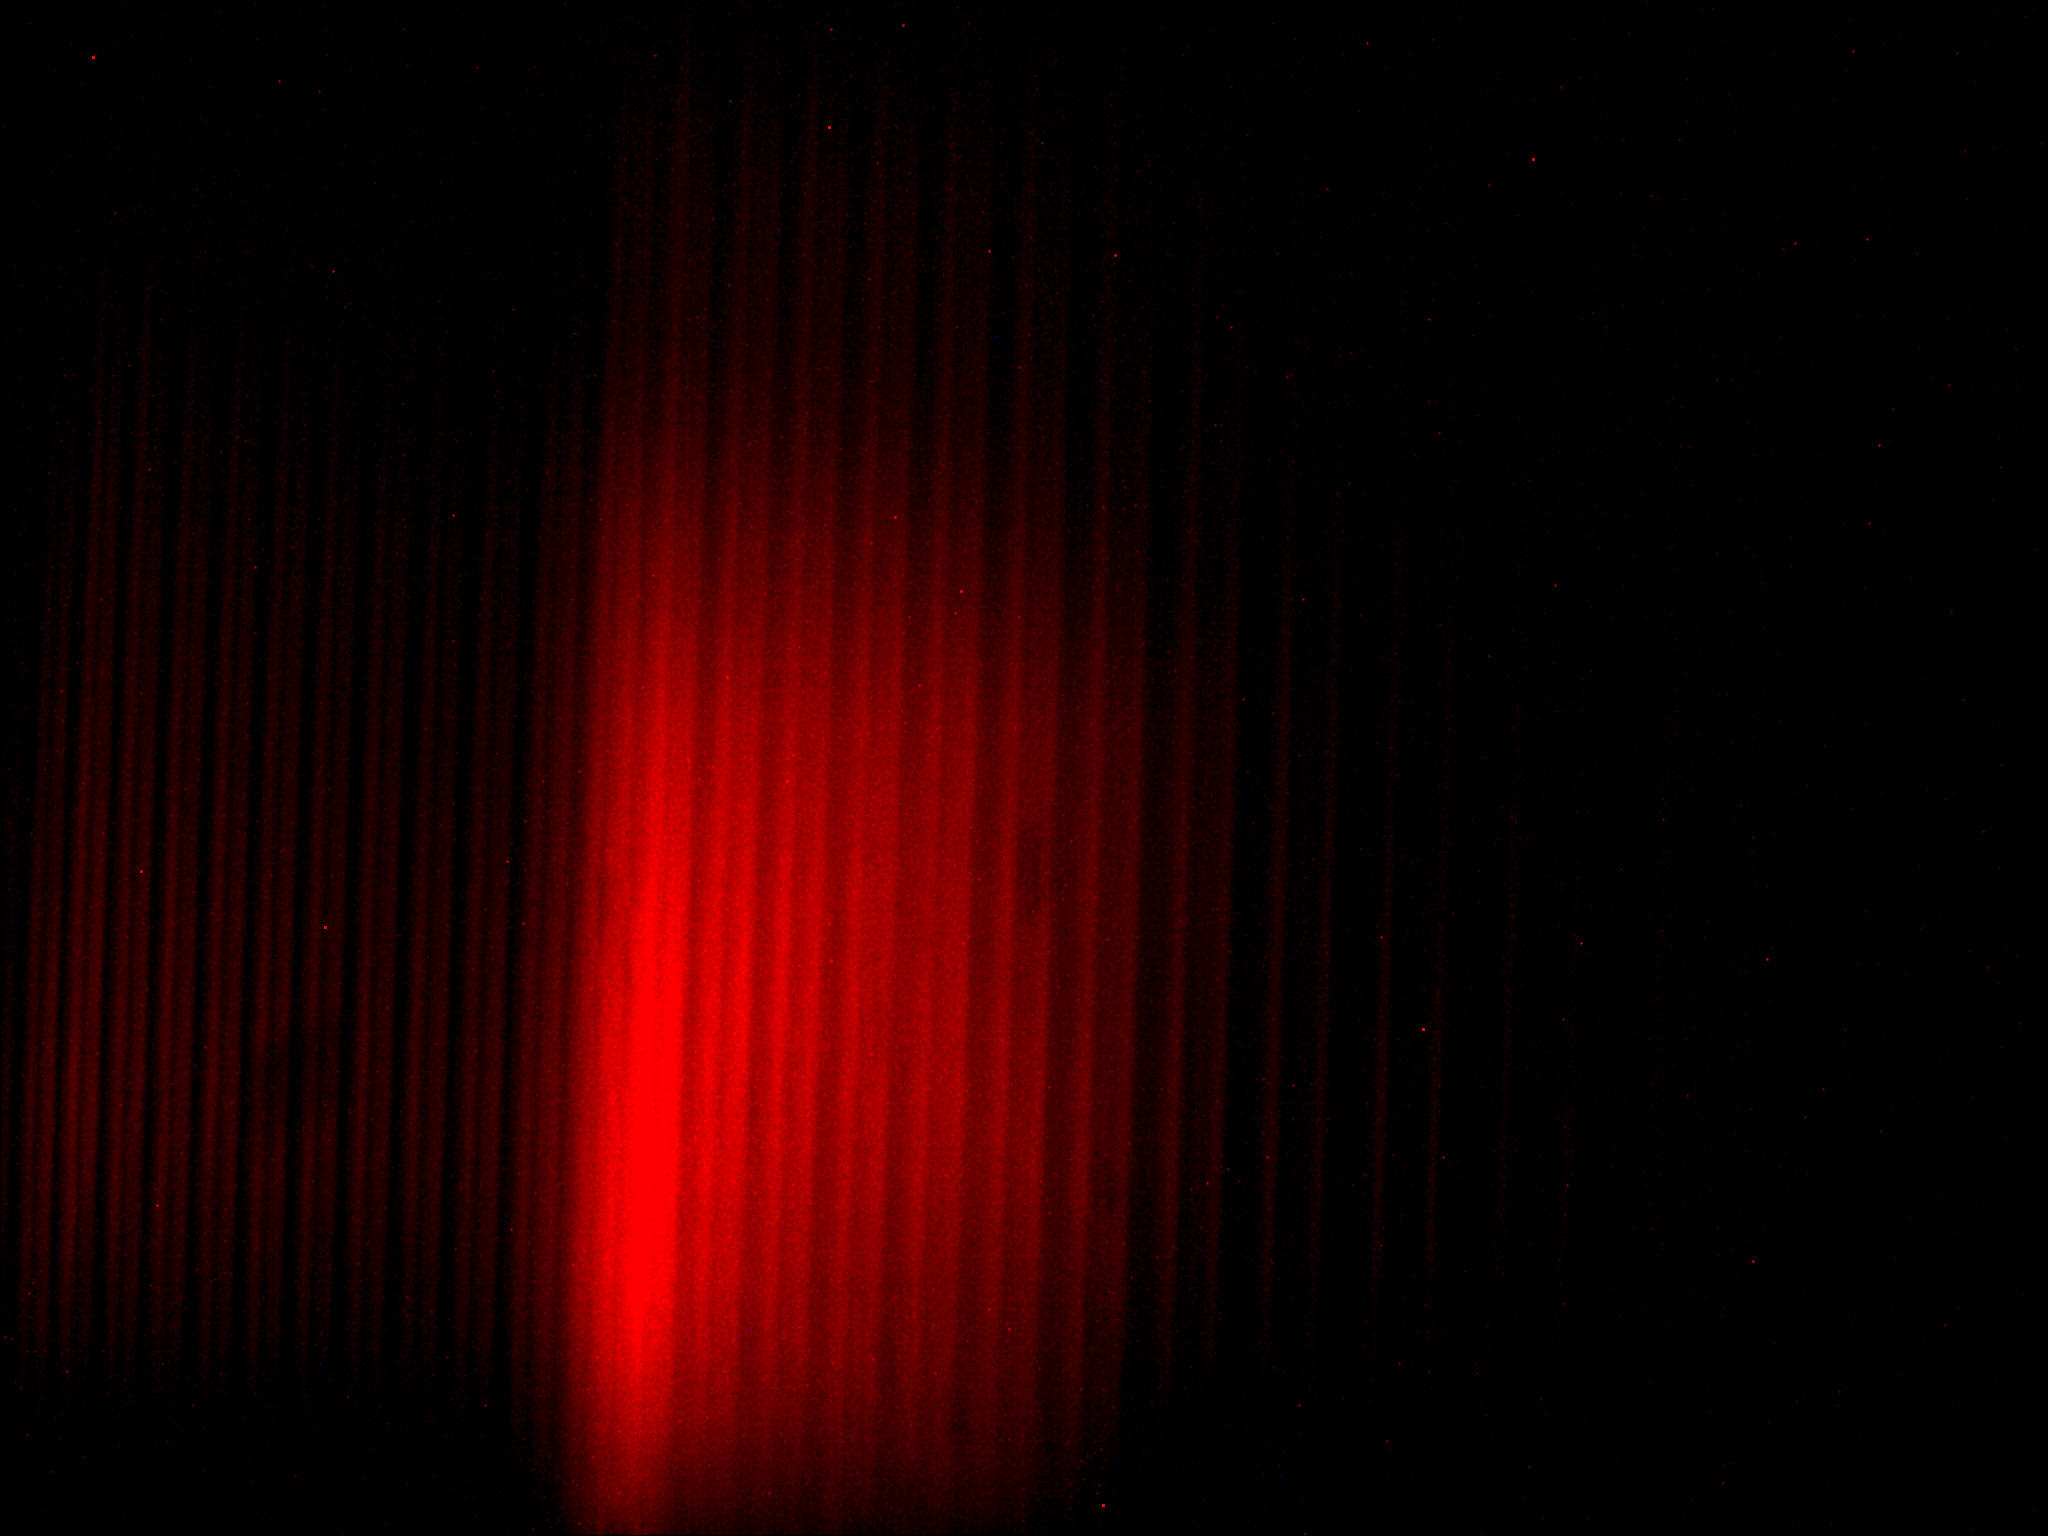
\includegraphics[width=.6\paperwidth, trim={0 300pt 0 900pt}, clip]{Auswertung/data/trans/10A/10A_sig}
        \caption{Beobachtete Linien in transversaler Ausrichtung, mit linearem Polarisationsfilter}
        \label{pic::3}
      \end{figure}

      Bei Variation der Stromstärke und des damit resultierenden Magnetfeldes, kann man beobachten, dass die Aufspaltung der Spektrallinien mit zunaehmender Stromstärke größer wird.

      \begin{figure}[H]
        \centering
        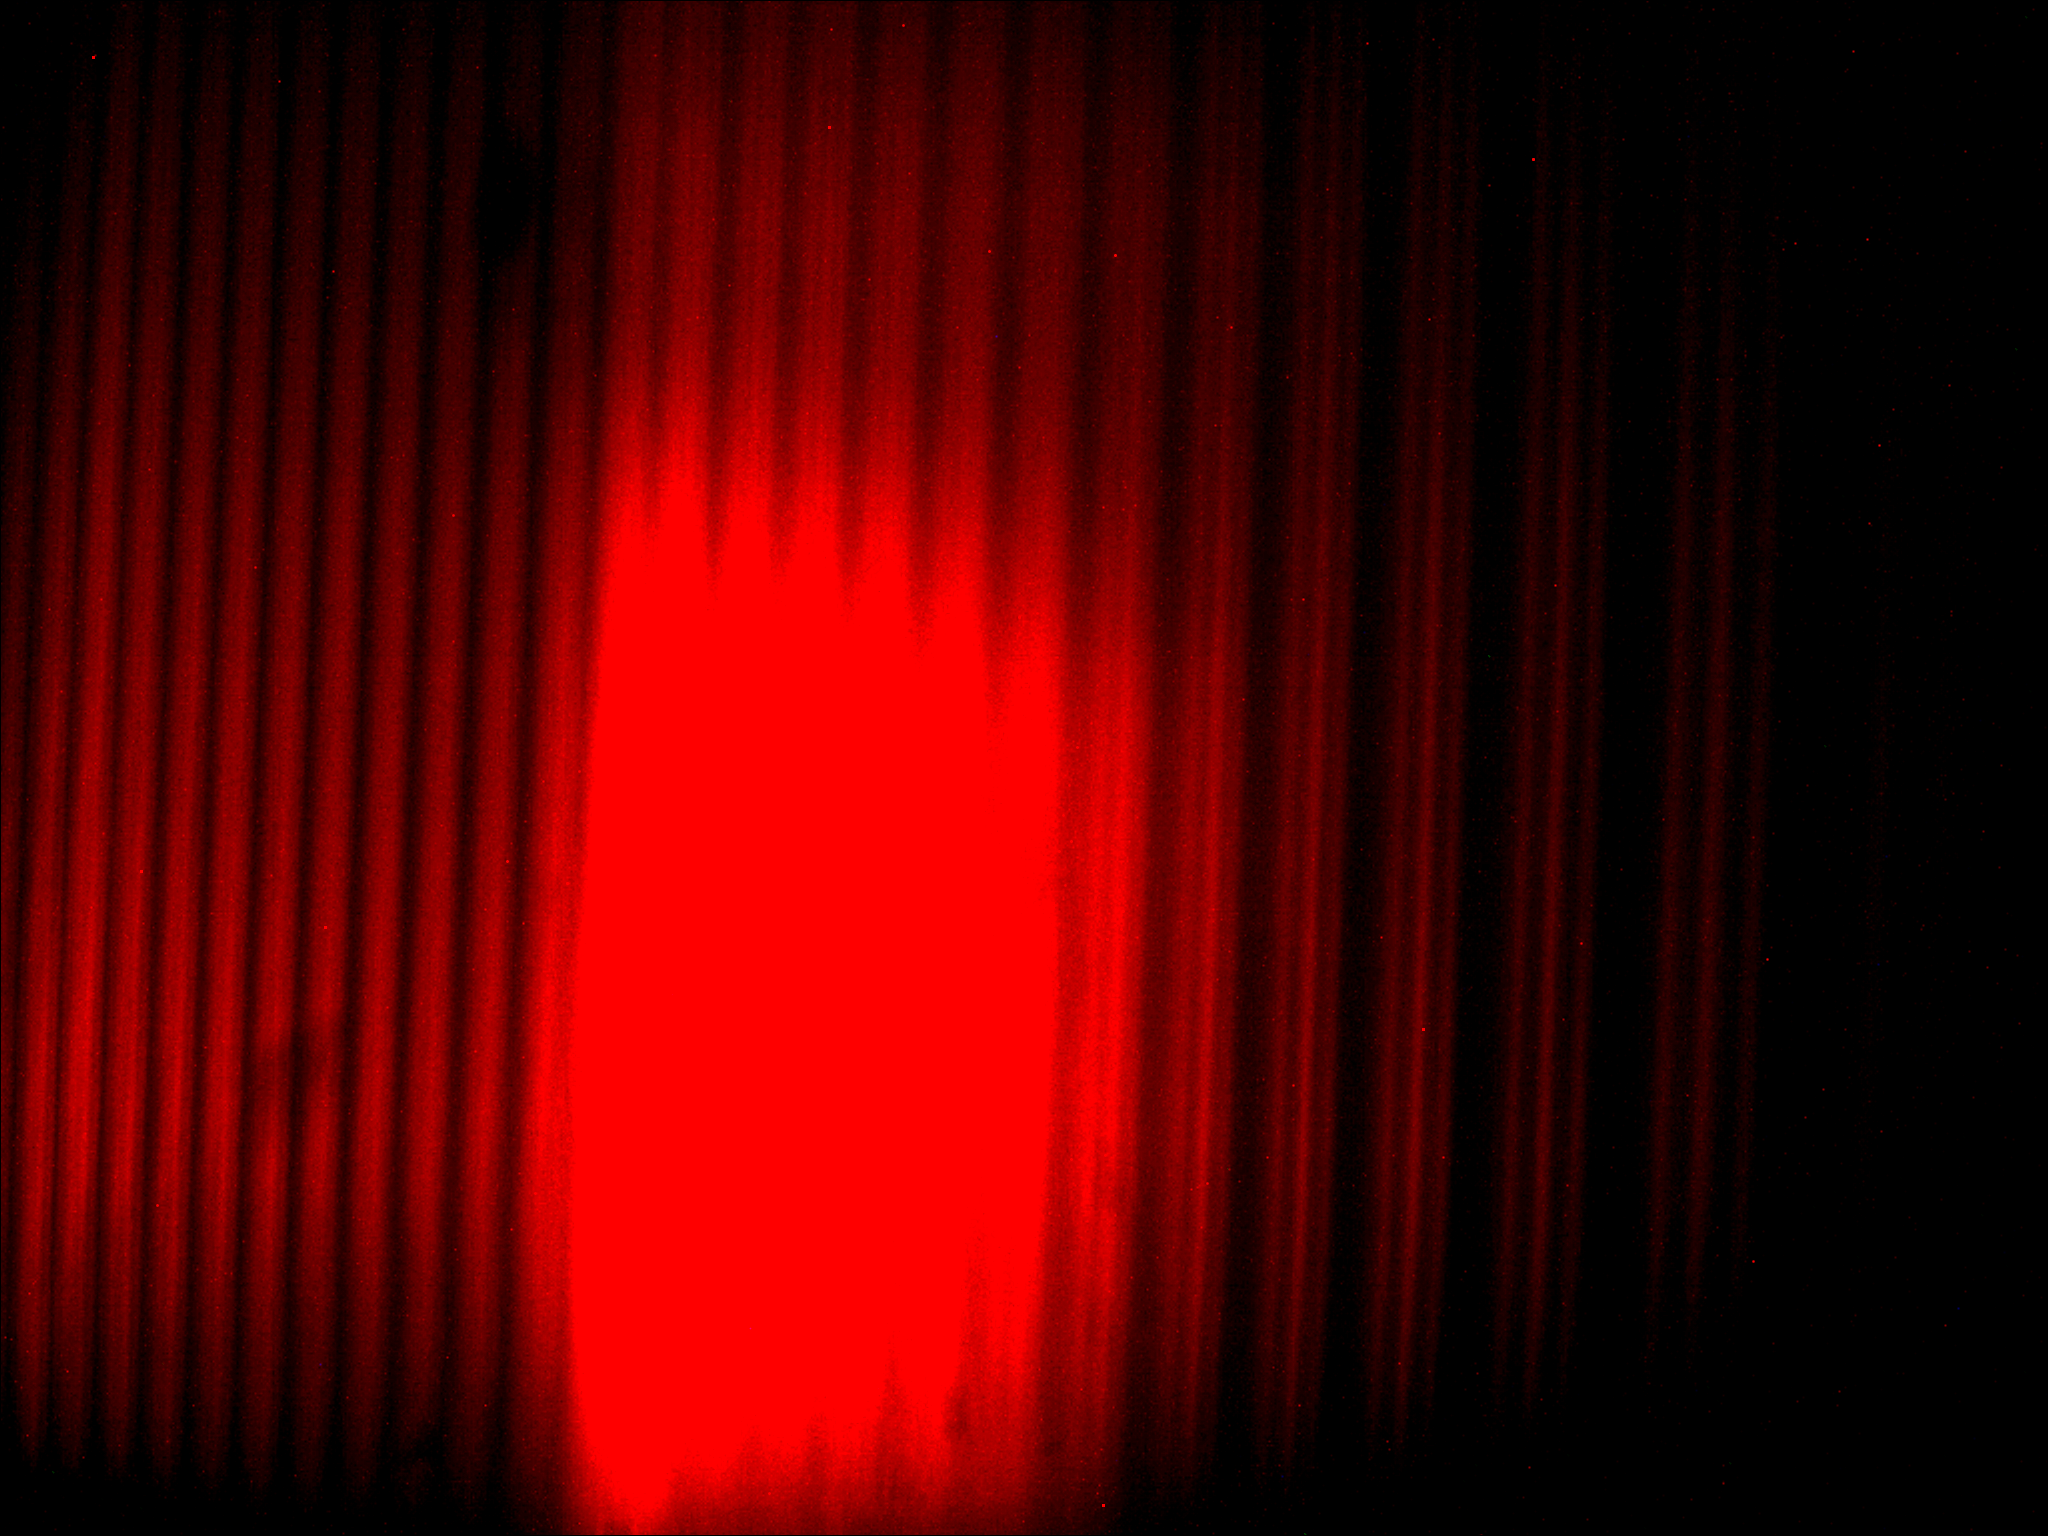
\includegraphics[width=.6\paperwidth,trim={0 600pt 0 500pt}, clip]{Auswertung/data/trans/10A/10A_l}
        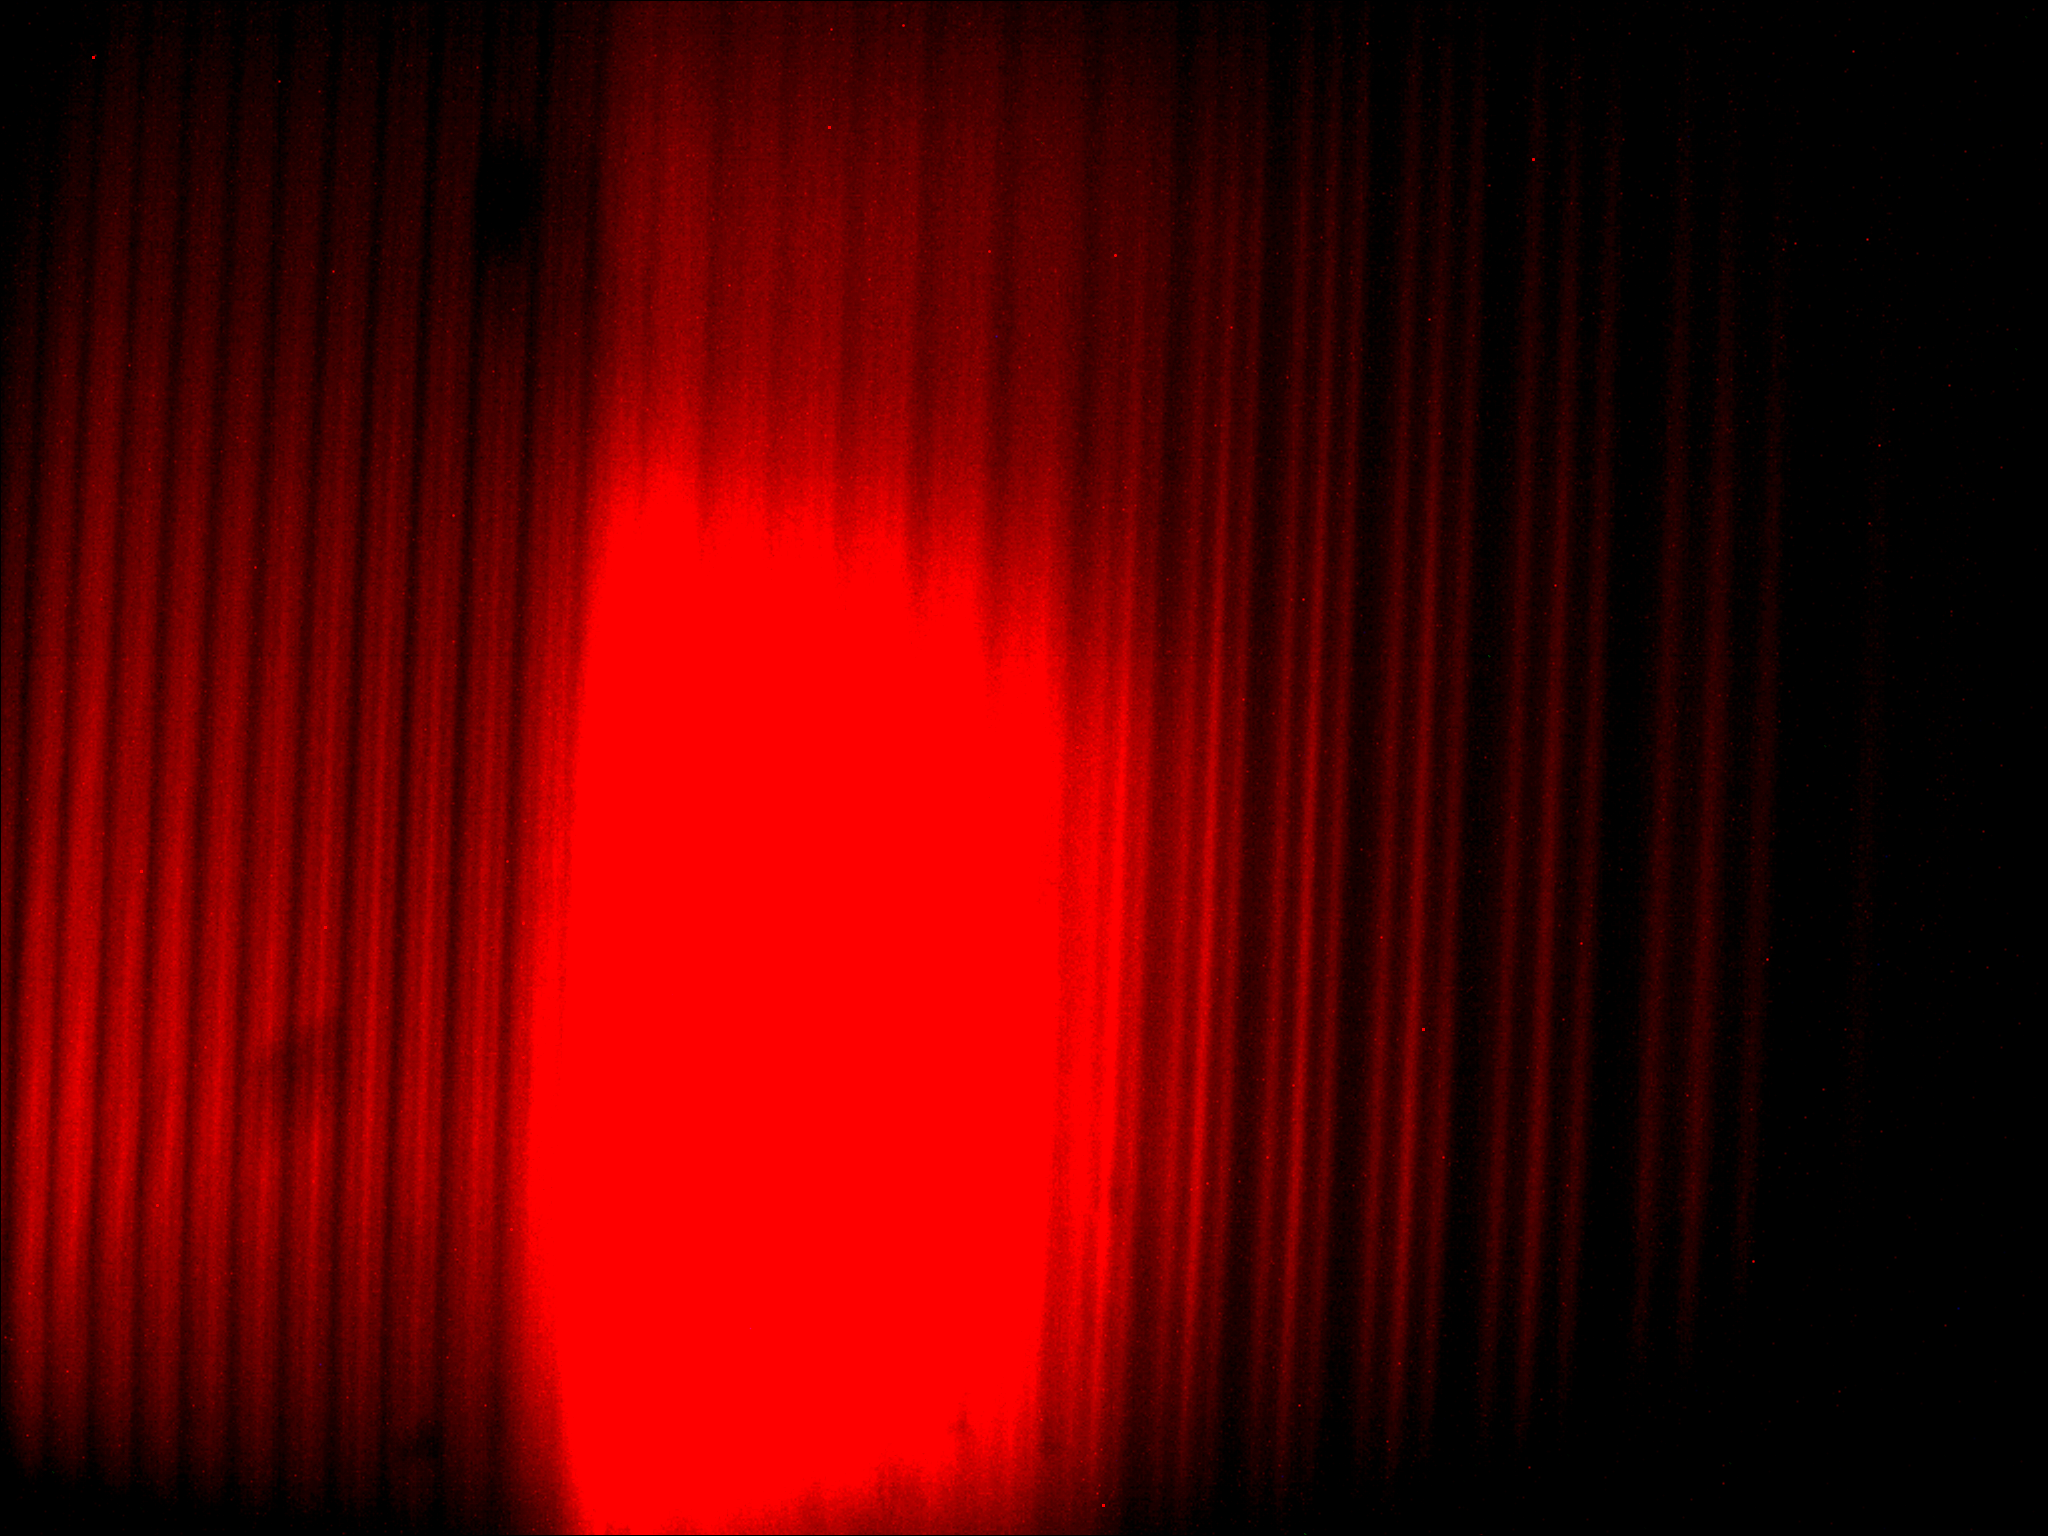
\includegraphics[width=.6\paperwidth,trim={0 200pt 0 900pt}, clip]{Auswertung/data/trans/13A/13A_l}
        \caption{Beobachtete Linien in transversaler Richtung, bei 10A (oben) und 13A (unten)}
        \label{pic::4}
      \end{figure}

    \subsection{Bestimmung der Wellenlängenverschiebung}
      \subsubsection{Position der $\pi$- und $\sigma$-Linien}
        Wir nutzen das Programm \textbf{JImage} um die zweidimensionalen Bilder der beobachteten spektralen Aufspaltung in eine eindimensionale Intensitätsverteilung zu konvertieren. Mit \textbf{Python} kann jetzt die Position (in Pixel) jeder $\pi$- und $\sigma$-Linie von etwa 5 Ordnungen (wegen der Reflektion in der Mitte der Bilder) pro Messung bestimmt werden.
        %TODO: add github repo refs

        Jeder gemessene Peak wird jetzt mit einer Gausskurve gefittet und daraus die Breite und Position bestimmt. Die Gaussfunktion berücksichtigt, dass durch die thermische Bewegung der Atome ein Doppler-Effekt entsteht und dadurch ist die ausgesandte Wellenlänge je nach Bewegungsrichtung des Atoms leicht verschoben, sodass die Linien im Vergleich zur Lorentz-Kurve breiter erscheinen. Als Fehler der Position wird hier der $\sigma^2$-Parameter der Gaussfunktion genutzt ($\Delta x = \sigma * 2.4 / 2$, also die halbe Halbwertsbreite).

        \begin{landscape}
          \thispagestyle{empty}
          \begin{figure}
            \vspace*{-2cm}
            \caption{Gefittete Positionen der Peaks}
            \hspace*{-6cm}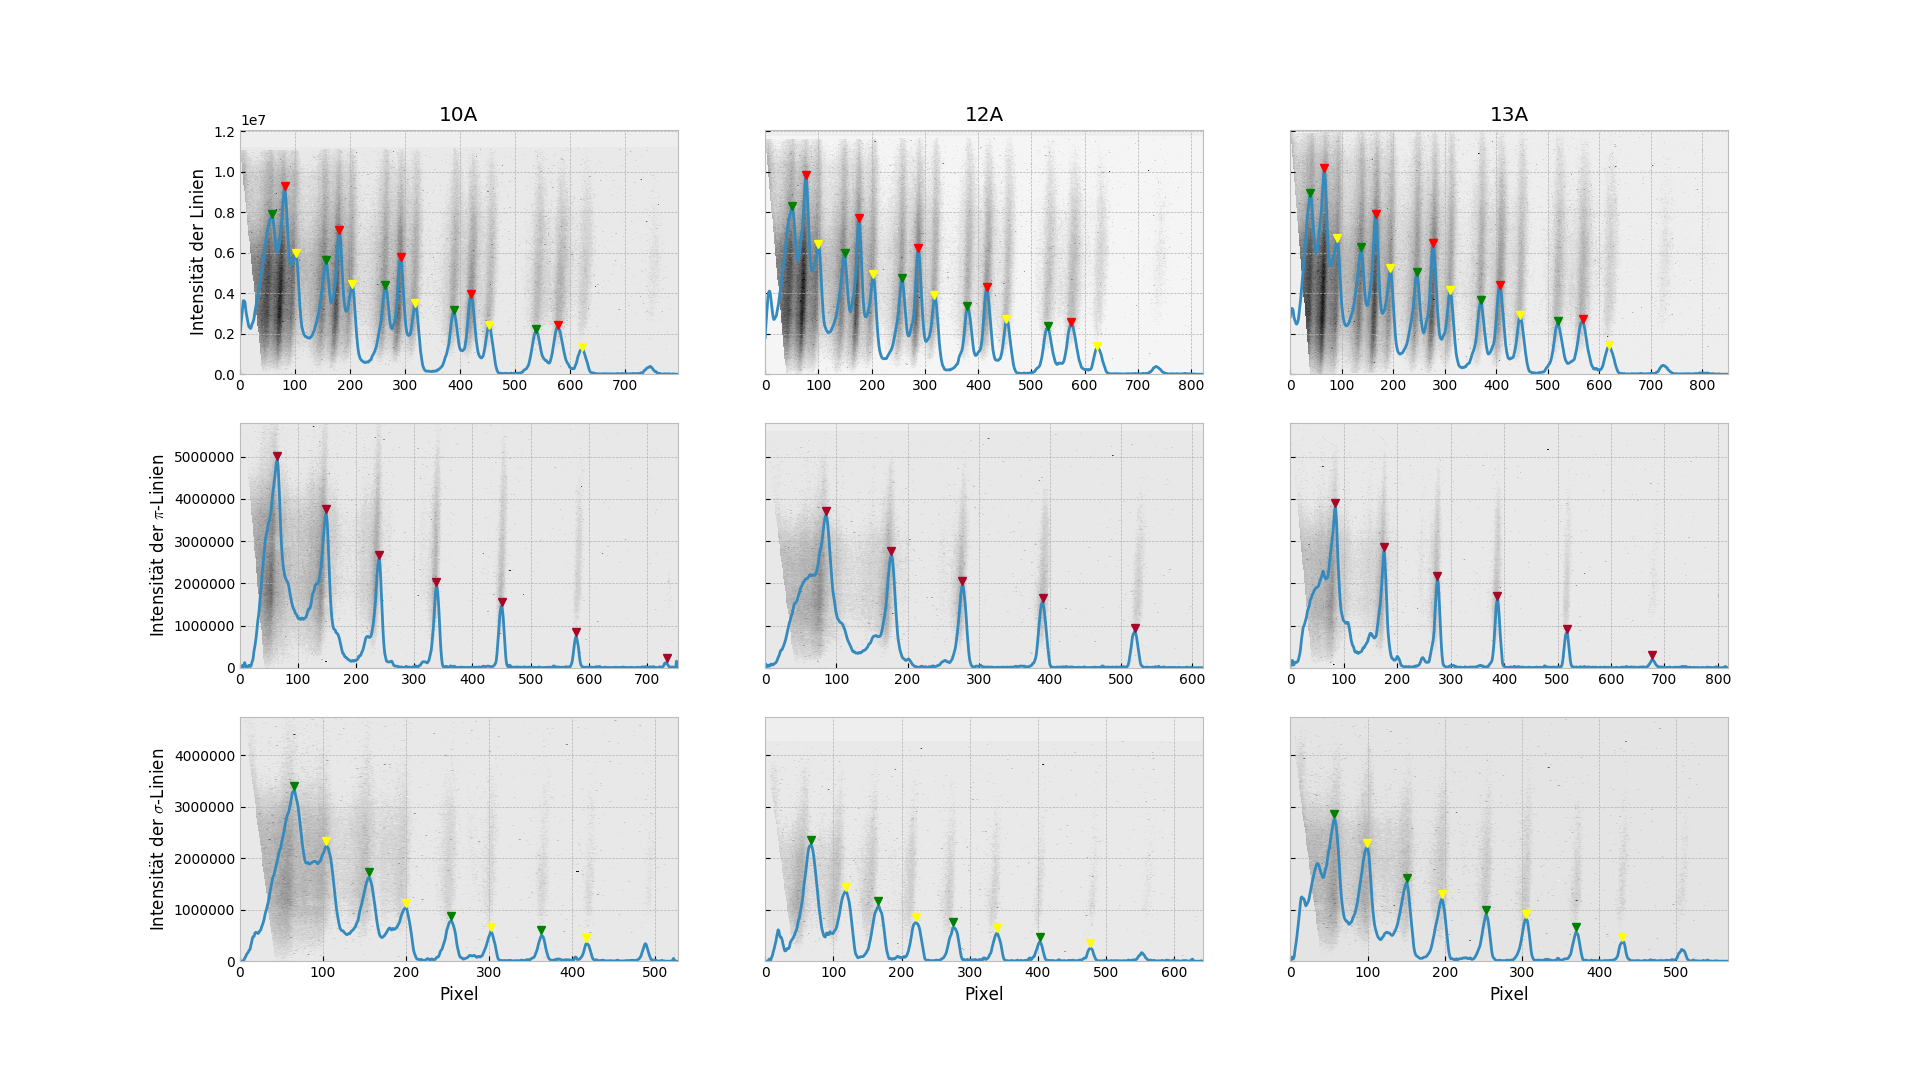
\includegraphics[width=1.5\paperwidth]{Auswertung/peaks}
          \end{figure}
        \end{landscape}

      \subsubsection{Verschiebung der Ordungen}
        Wir ordnen nun den $\pi$-Linien nun Ordnungszahlen zu, diese sollten nur diskrete, ganzzahlige Werte sein, allerdings möchten wir den $\sigma$-Linien auch eine solche Ordnung zuordnen, also betrachten wir eine kontinuierliche Fitfunktion. In unserem Fall ist diese eine Polynomfunktion 2.Grades (s. \hyperref[plot::2]{Abb. \ref*{plot::2}}). Diese Näherung ist innerhalb unserer Näherung ausreichend, da ein Polynom höheren Grades keine signifikante Verbesserung der Beschreibung unserer Daten liefert.

        Um die Fehler der Beugungsordnung zu bestimmen nutzen wir:
        \begin{align}
          \Delta k(a) = k(a+\Delta a) - k(a)
        \end{align}
        wobei die Fehler der Fitparameter vernachlässigt werden. $a$ ist hier die Position der Linien in Pixel, $k$ die zugeordnete Beugungsordnung. Jetzt werden die Verschiebungen der $\sigma$-Linien zur zugehörigen $\pi$-Linie, in Bruchteilen einer Beugungsordnung, berechnet und geplottet (\hyperref[plot::3]{Abb. \ref*{plot::3}})

        \begin{landscape}
          \thispagestyle{empty}
          \begin{figure}
            \vspace*{-2cm}
            \caption{Polynomfits für die drei Stromstärken}
            \hspace*{-5cm}
            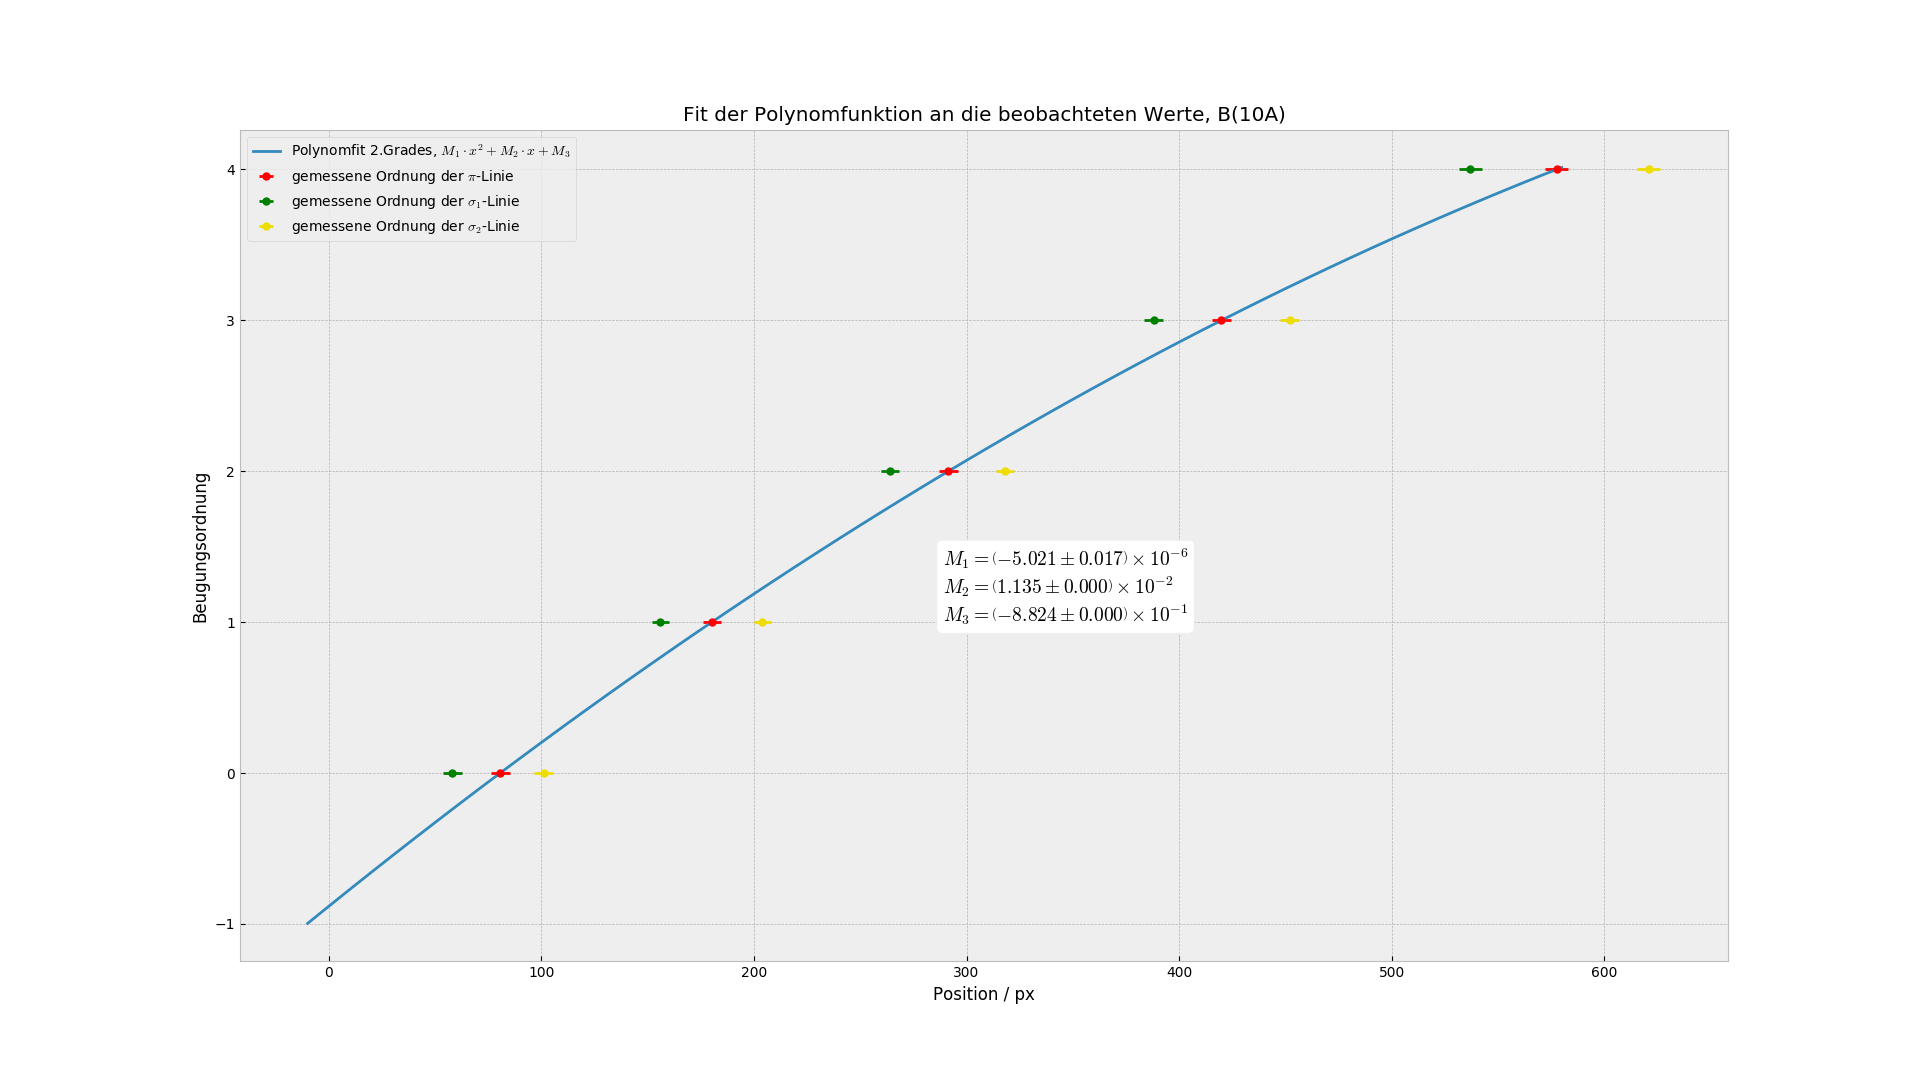
\includegraphics[width=.45\paperwidth]{Auswertung/scatterorder/sco_10A}
            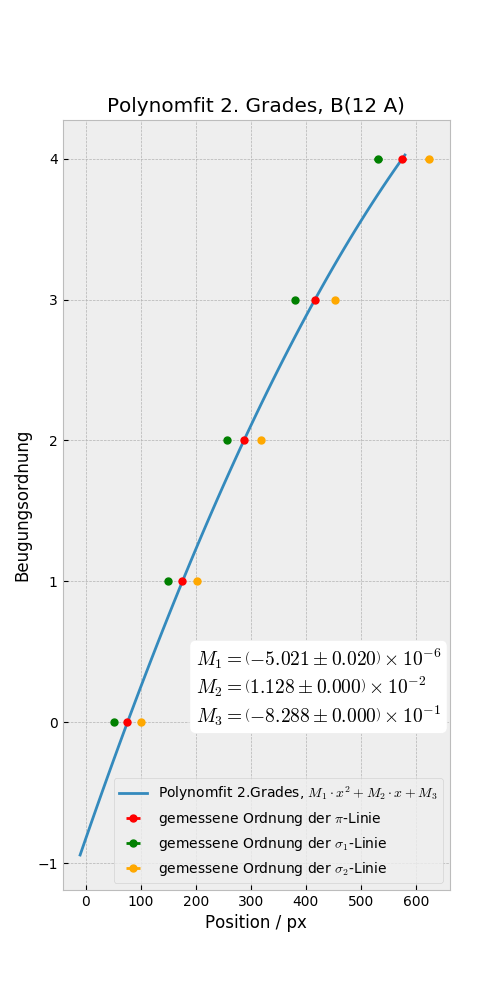
\includegraphics[width=.45\paperwidth]{Auswertung/scatterorder/sco_12A}
            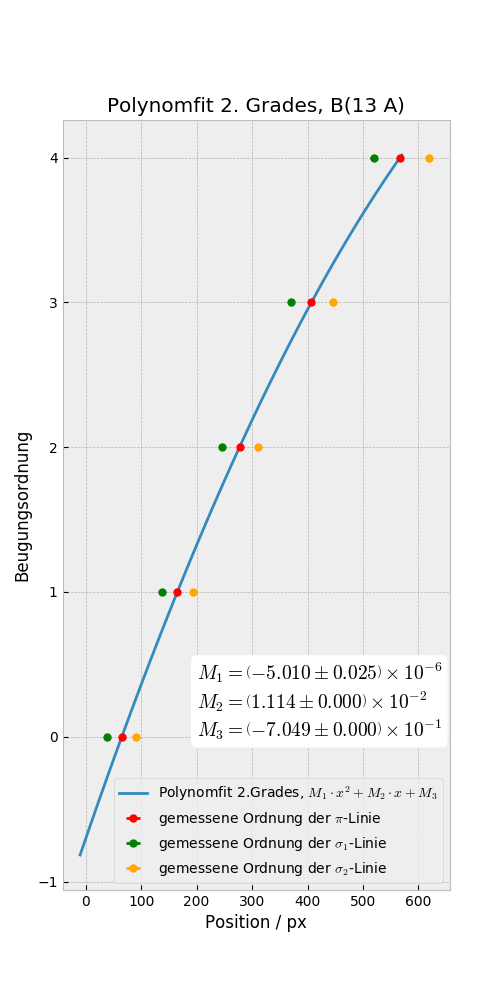
\includegraphics[width=.45\paperwidth]{Auswertung/scatterorder/sco_13A}
          \end{figure}

          \thispagestyle{empty}
          \begin{figure}
            \vspace*{-2cm}
            \caption{Verschiebung der Beugungsordnung}
            \hspace*{-5cm}\vspace{-1cm}
            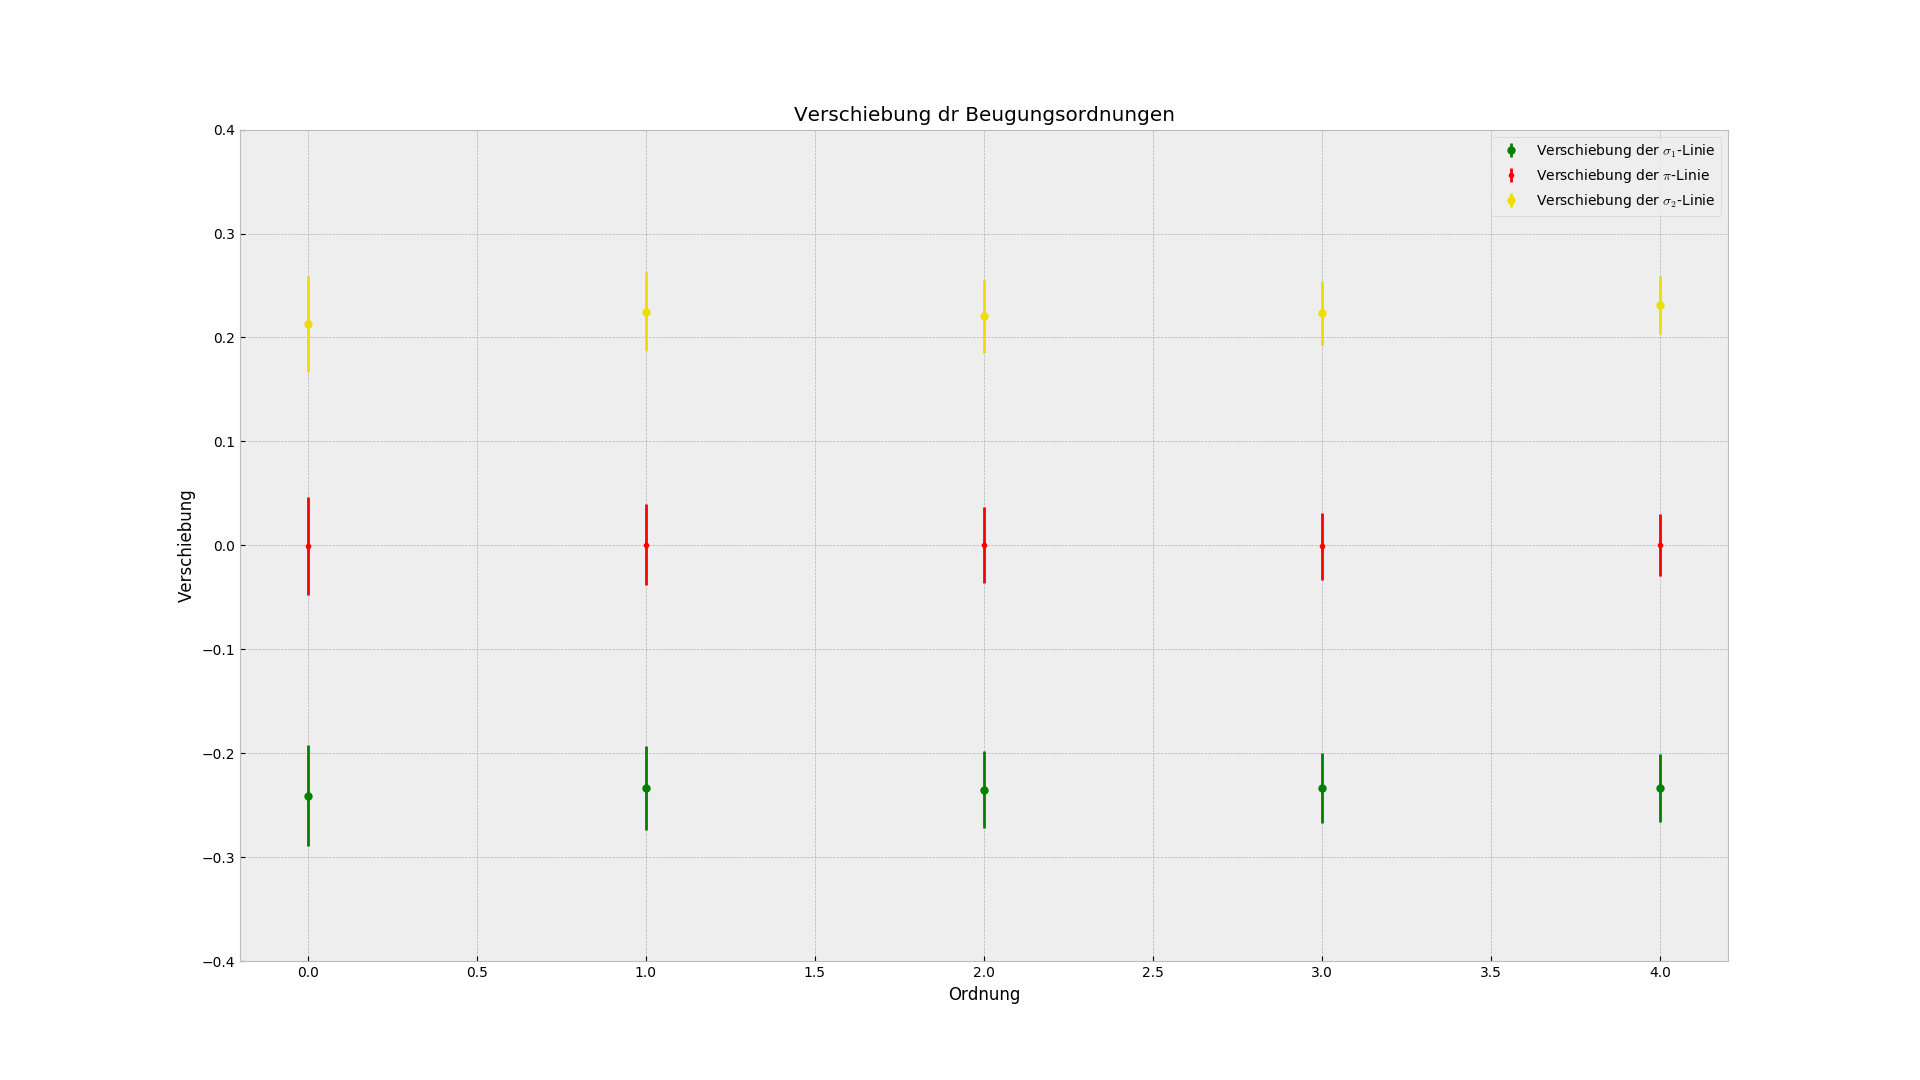
\includegraphics[width=.45\paperwidth]{Auswertung/scatterorder/diff_sco10A}
            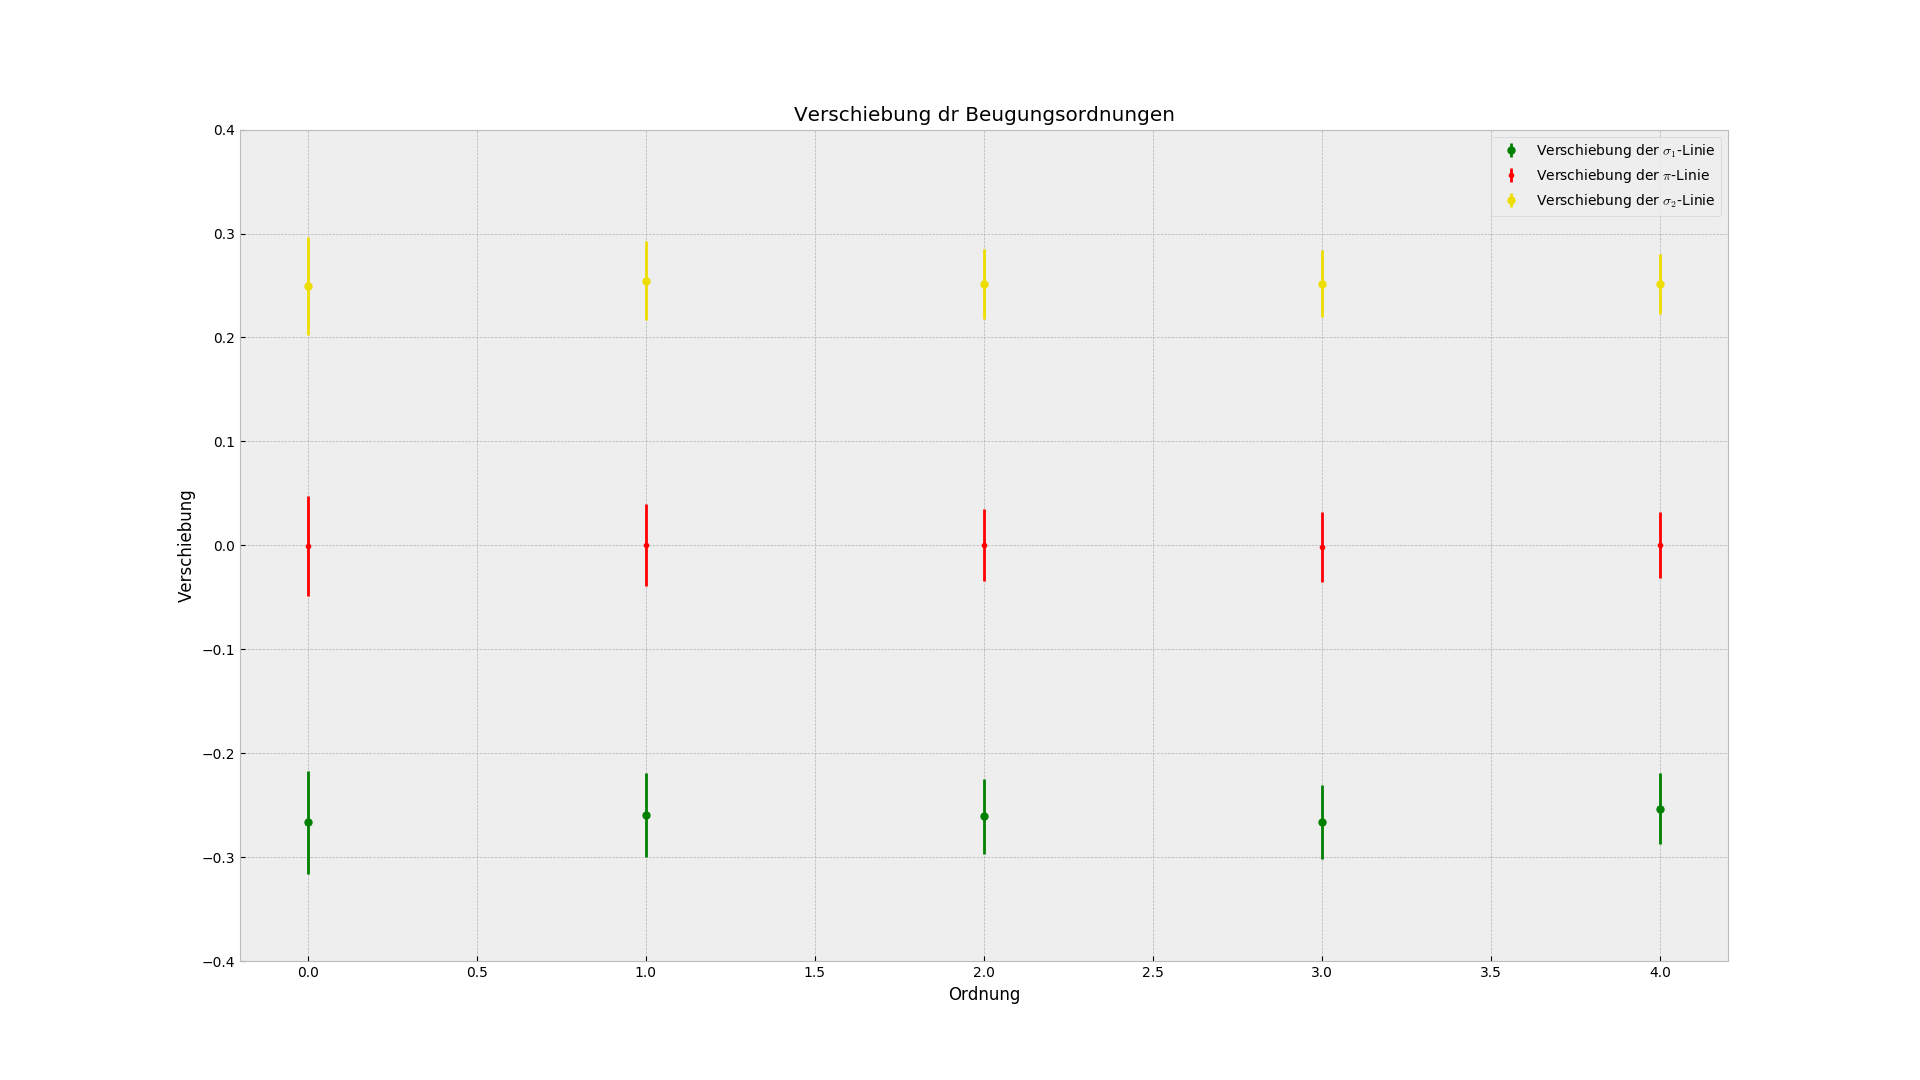
\includegraphics[width=.45\paperwidth]{Auswertung/scatterorder/diff_sco12A}
            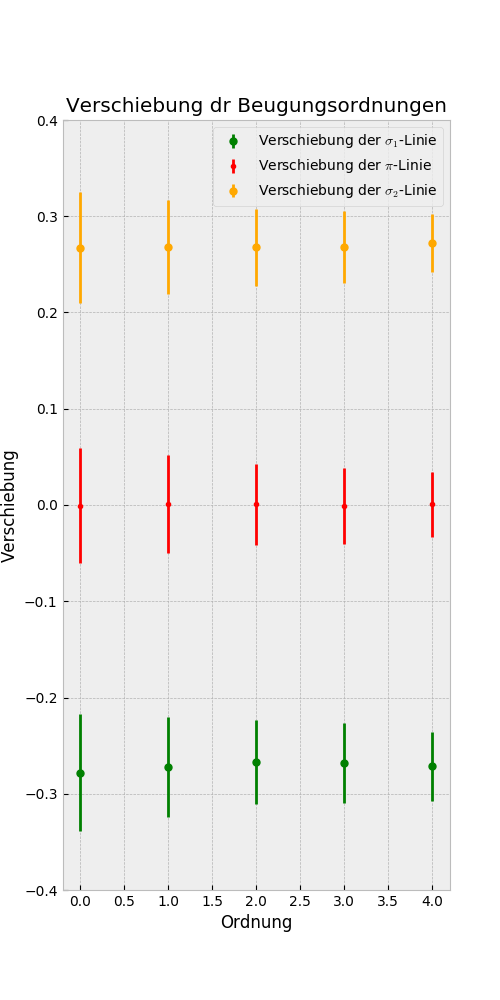
\includegraphics[width=.45\paperwidth]{Auswertung/scatterorder/diff_sco13A}
          \end{figure}
        \end{landscape}
